\icode{E-EXM-FI-L3-260625-001}
小明在实验室探究物体加速度与所受合外力的关系，实验装置如图甲所示，主要实验步骤如下：

\begin{minipage}[c]{.45\textwidth}
    \centering
    \begin{tikzpicture}[scale=1.2,font=\scriptsize]
        \draw[fill=orange!70] (0,-.1) rectangle(4,0) (.5,-.1) rectangle(.8,-1) (3.5,-.1) rectangle(3.2,-1);
        \draw[fill=black] (.4,0) rectangle(.5,.3);
        \draw (.4,.5)..controls(0,.5)and(-.2,.2)..(-.5,0);
        \filldraw[fill=gray,rotate around={-5:(3.9,0)}] (0.2,0) rectangle(3.9,.1);
        \filldraw[fill=white,rotate around={-5:(3.9,0)}](.3,.1) rectangle(.6,.25) (2,.2) rectangle(2.5,.35);
        \draw[purple,rotate around={-5:(3.9,0)}] (.6,.25)--(2,.25) (2.5,.25)--(4.1,.25);
        \filldraw[fill=white,rotate around={-5:(3.9,0)}] (2.1,.15) circle(.05) (2.4,.15) circle(.05);
        \filldraw[fill=white,rotate around={18:(3.9,0)}] (3.9,0.05) rectangle(4.15,.1);
        \draw (4.1,.13) circle(.1);
        \fill (4.1,.13) circle(.05);
        \draw[purple] (4.2,.13)--(4.2,-.5);
        \draw (4.1,-.5) rectangle(4.3,-.7);
        \node at(4.2,-.9) {钩码};
        \node at(2.3,.6)[rotate=-5]{小车};
        \node at(.5,.7)[rotate=-5]{打点计时器};
        \node at(-.3,.2)[left]{纸带};
        \node at(.8,.15){木板};
    \end{tikzpicture}
\end{minipage}
\begin{minipage}[c]{.49\textwidth}
    \centering
    \begin{tikzpicture}[>=latex,font=\scriptsize]
        \draw[->,blue] (0,0)--(3,0)node[below]{\(n\)};
        \draw[->,blue] (0,0)--(0,2.7)node[right]{\(\frac{1}{a}\)/(\,\qty{}{s^2\cdot m^{-1}})};
        \draw[purple] (0,.8)node[left]{\(b\)}--(2.3,2.3);
        \node at(-.2,-.2)[blue]{\(O\)};
    \end{tikzpicture}
\end{minipage}

\begin{figure}[htbp]
    \centering
    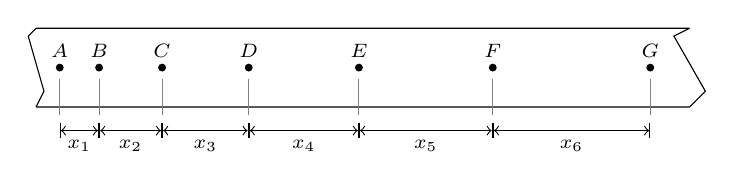
\begin{tikzpicture}[font=\scriptsize]
    \draw (-.3,.5)--(8,.5) (-.3,-.5)--(8,-.5) (-.3,.5)--(-.4,.4)--(-.2,-.3)--(-.3,-.5) (8,.5)--(7.8,.4)--(8.2,-.3)--(8,-.5);
    \foreach \x in{0,.5,1.3,2.4,3.8,5.5,7.5}
        \draw[gray] (\x,-.15)--(\x,-.6);
    \foreach \x/\c in{0/A,.5/B,1.3/C,2.4/D,3.8/E,5.5/F,7.5/G}
        \fill (\x,0)node[above]{\(\c\)} circle(.05);
    \foreach \x/\y/\n in{0/.5/x_1,.5/1.3/x_2,1.3/2.4/x_3,2.4/3.8/x_4,3.8/5.5/x_5,5.5/7.5/x_6}
        \draw[|<->|] (\x,-.8)--node[below]{\(\n\)}(\y,-.8);
\end{tikzpicture}
\end{figure}

（1）调整长木板倾角进行阻力补偿，使小车恰好沿长木板向下做匀速运动。

（2）保持长木板的倾角不变，绳子下端只挂一个钩码，将小车移近打点计时器，接通电源然后释放小车，小车沿长木板向下做匀加速直线运动，得到一条纸带如图所示，\(A\)、\(B\)、\(C\)、\(D\)、 \(E\)、\(F\)、\(G\)为计数点，相邻计数点间还有4个点未画出，打点计时器的频率为\,\qty{50}{Hz}。利用刻度尺测量得到\(x_1 =\) \,\qty{2.19}{cm}，\(x_2 =\) \,\qty{2.76}{cm}，\(x_3 =\) \,\qty{3.35}{cm}，\(x_4=\) \,\qty{3.93}{cm}，\(x_5 =\) \,\qty{4.58}{cm}，\(x_6 =\) \,\qty{5.20}{cm}。通过纸带求得小车在\(C\)点的速度大小为\underline{\hbox to 4em{}}\,\qty{}{m/s}；通过纸带求得小车加速度大小为\underline{\hbox to 4em{}}\,\qty{}{m/s^2}。（均保留2位有效数字）
  
（3）保持绳子下端悬挂的钩码不变，在小车上放置不同数量的相同钩码，小车上钩码的个数记为\(n\)，重复实验操作（2），求出小车对应的加速度\(a\)，得到加速度的倒数\(\frac{1}{a}\)和钩码个数\(n\)的\(\frac{1}{a} - n\)图像如图所示，已知一个钩码的质量为\(m_0\)，图像中直线斜率为\(k\)，纵轴截距为\(b\)，利用题中信息可得出重力加速度\(g =\)\underline{\hbox to 6em{}}，小车的质量\(M =\)\underline{\hbox to 8em{}}。（用\(k\)、\(b\)、\(m_0\)表示）。